
% Take extra care in avoiding ``expansion'' -- stick to ``evaluation''

\begin{abstract}
Despite the recent improvements in admissible heuristic search techniques
in classical planning, it is known that the the exponential growth of
search plateau in A* is unavoidable even under the optimistic assumption.
 % 
We investigate various existing myth on tiebreaking
strategies and propose simple yet effective methods for improving the
search performance within plateau.
 % 
 % 
 They do not depend on any particular heuristic, nor
 on multi-heuristic portfolio.
 They work even if the heuristic
 function no longer provides useful information.
 % Moreover, they do not even try to obtain any further information from
 % the domain.
 We empirically evaluate our strategies against state-of-the-art admissible planner.
\end{abstract}

\section{Introduction}
%Motivation: The Importance of the Last Frontier in A* and Domains with Large Plateaus
\label{sec-1}



%\subsubparagraph{\astar and perfect heuristics}

This paper investigates tie-breaking strategies for \astar.
\astar is a standard search algorithm for finding an optimal-cost path 
from an initial state $s$ to some goal state $g \in G$ in a search space represented as a graph \cite{hart1968formal}.
In each iteration, \astar selects and \emph{expands} a node $n$ from the OPEN priority queue.
$n$ is the node which has the lowest $f$-cost in OPEN, where for node $n$, $f(n)$ is the sum of  $g(n)$, the cost of the current path from the start state to $n$, and $h(n)$, a heuristic estimate of the cost from $n$ to a goal state.
\astar returns an optimal solution when $h$ is admissible, i.e., when it
never overestimates the true distance to the goal $h^*$.

In order to guarantee solution optimality, \astar expands all
nodes with $f(n) < f^*$, where $f^*$ is the cost of the optimal solution.
%All nodes with $f(n) = k$ are expanded before any node with $f(n) > k$ are expanded.
%Thus, after all nodes with $f(n) < f^*$ have been expanded, 
\astar expands \emph{some} of the nodes with $f(n) = f^*$, and never expands a node with $f(n) > f^*$.
Thus, the \emph{effective search space of \astar}, $N$, is the set of nodes with 
$f(n) \leq f^*$, and
much of the work in the AI search and planning literature  has focused on reducing the size of $N$ by
developing more accurate, admissible heuristic functions.

In many problems, the size of the \emph{last frontier}, the set of nodes with $f(n)=f^*$, accounts for a significant portion of $A$.
\refig{fig:plateau-noh} plots the number of states with $f(n) = f^*$ (y-axis)
versus the number of states with $f(n) \leq f^*$
for a set of 1104 benchmark problem instances from the ICAPS International Planning Competition (IPC1998-2011).
For many instances in \refig{fig:plateau-noh},  a large fraction of the nodes with $f(n) \leq f^*$ have $f(n)=f^*$.
For example, in the Openstacks domain, almost all states with $f(n) \leq f^*$ have cost $f^*$.
In such domains, the behavior of \astar on the last frontier is critical -- the policy for deciding which nodes to expand in the last frontier can have a significant impact on the performance of \astar.

\begin{figure}[htb]
 \centering \relsize{-3} 
 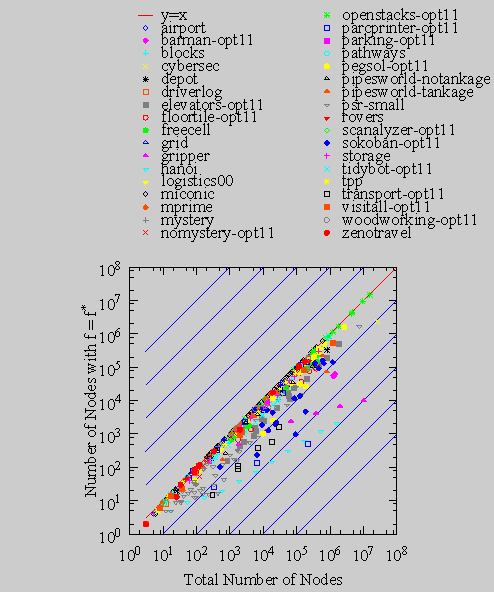
\includegraphics{tables/aaai16-frontier/aaai16prelim3/lmcut_frontier_noh-front.pdf}
 \caption{
 The number of the nodes with cost $f=f^*$ (y-axis) compared to the
 total number of nodes in the search space with cost $f\leq f^*$ on 1104 IPC benchmark problems
(search space analyzed using Fast Downward with \lmcut heuristic, slightly modified to generate all nodes with cost $f^*$).}
\label{fig:plateau-noh}
\end{figure}

In this paper, we focus on the \emph{tie-breaking} policy used by
\astar, which selects a node to expand among nodes with the same
$f$-cost.  Since \astar expandes all nodes with $f$-cost less than $f^*$
before expanding any nodes with cost $f^*$, the tie-breaking poicy only
affects performance when considering the last frontier (nodes with cost
$f^*$).  \todo[Although there has not been much previous \emph{in-depth} work
on tie-breaking policies]{mention vallati and ``Merrier''}, it is widely believed that among nodes with
cost $f(n) = f^*$, ties should be broken according to $h(n)$, i.e.,
nodes with smaller $h$ values should be expanded first.  While this is a
useful rule of thumb in many domains, it turns out that tie-breaking
requires more careful consideration, particularly for problems with
large \emph{plateaus} -- regions of the search space with the same $f$-cost.
\emph{Note that all tiebreaking strategies investigated in this paper
maintain the admissibility of the search because it only affects the node expansion
order among the nodes with the same $f$-cost.}

We first empirically clarify two facts regarding the
existing tiebreaking strategy for \astar as follows.
% 
First, in implementing the open list of \astar, priority queue which holds
\lifo-buckets for each $f$ tends to be more efficient than that holds \fifo-buckets.
% 
Second, with \lifo-based implementation, $h$-based tiebreaking which
frequently appears in the heuristic search literatures have little
impact on the performance.
% 
%% Remove?
% \todo[
% Third, the \lifo-based bucket implementation and $h$-based tiebreaking
% both share the greedy search pattern within the plateau of the
% search space.]{this is not shown yet. how to show it? xy-plot of the node
% evaluation order?}
 
Next, we propose three tiebreaking methods
based on the \emph{depth} within the plateau, and
we show that the depth-based tibreaking in the plateau is
the principal factor of the performance which is
not affected by the particular action ordering in the domain definition.
% 
With this result, we also show that 
the performance of above \lifo tiebreaking can be explained by its
depth-first strategy, and its machine-level efficiency of \lifo
has little effect on the performance.
% 
We also show that,
although the performances of the depth-based tiebreaking
methods are not affected by the
different action orderings of the same domain definition,
three tiebreaking methods perform differently on different domains,
with no clear dominance relationship among domains.

Finally, based on the absence of dominance relationship, we propose a
new class of portfolio strategy called \emph{Low Overhead Portfolio} (LOP),
which alternates between several depth-based tiebreaking methods.
Unlike the simple alternating open list proposed in LAMA planner \cite{richter2010lama},
it prevents the interaction between the queues and maintains the original
expansion order of each queue, allowing a clear theoretical analysis.
Also, it targets a single-heuristics, multi-tiebreaking scenario, unlike
the multi-heuristic scenario assumed in LAMA's alternating open list.
% 
LOP has several interesting characteristics:
First, the number of evaluations of nodes with $f<f*$ with LOP is exactly the same as
those with any single tiebreaking strategy.
Also, it has a theoretical guarantee that
the number of evaluations of nodes with $f=f*$ is at most $N$ times the \emph{minimum} 
of the evaluations required by $N$ strategies in the portfolio.
% 
%%% removed, we curretntly do not have much clue
% To put it simply, this portfolio does not need additional computation
% and we get a speedup for free (aside from the negligeble differences).
% Also, it is characteristic in that it works with a single heuristic function.
% We also empirically evaluates LOP.

\section{Tie-breaking Strategies in \astar}

%Aside from the heuristic function, most best-first family of search
%algorithms, including \astar, IDA* and so on, have a tiebreaking criteria which is used
%when two nodes have the same $f$ value.

If multiple nodes with the same $f$-cost are possible, \astar
must implement some tie-breaking policy (either
explicitly or implicitly) in order to select from among these nodes.
The early literature on heuristic search seems to have been mostly agnostic on the issue of tie-breaking.
The original paper proposing \astar paper, as well as Nilsson's
subsequent textbook states: ``Select the open node $n$ whose value $f$
is smallest. Resolve ties arbitrarily, but always in favor of any [goal
node]'' \cite[p.102 Step 2]{hart1968formal} \cite[p.69]{Nilsson71}.
% Although it is possible to interpret this to imply $h$-based tie-breaking
% since goal nodes are the special case where $h=0$,
% they make no further metion of tie-breaking.
Pearl's seminal textbook on search specifies that best-first search should ``break ties arbitrarily'' (\citeyear{pearl1984heuristics}, p.48, Step 3), but does not specifically mention tie-breaking for \astar.
Interestingly, in his analysis of IDA*, Korf mentions that ``If \astar employs the tie-breaking rule of 'most-recently generated', it must also expand the same nodes [as IDA*]'' (\citeyear{korf1985depth}) -- this last-in-first-out ordering is the first explicit mention we found of a tie-breaking policy not based on $h$.

In recent years, tie-breaking accoording to $h$-values has become ``folklore'' in the search community.
\citeauthor{hansen2007anytime} state that ``It is well-known 
that \astar achieves best performance when it breaks ties
in favor of nodes with least h-cost'' \cite{hansen2007anytime}.
\citeauthor{holte2010common} writes ``\astar breaks ties in favour
of larger g values, as is most often done'' (note that since $f=g+h$, preferring large $g$ is equivalent to preferring smaller $h$).
% \citeauthor{felner2011inconsistent} also assume ``ties are broken in
% favor of low h-values'' in describing Bidirectional Pathmax for \astar.
In their detailed survey/tutorial of efficient \astar implementations, \citeauthor{burns2012implementing} also break ties ``preferring high
$g$.'' They further write: ``The reasoning is that the goal can be found more quickly in the final $f$ layer of search''. 
Thus, tie-breaking according to $h$-values appears to be ubiquitous in practice.


Although the standard practice of tie-breaking according to $h$ might be sufficient in some domains, further levels of tie-breaking (explicit or implicit) are required if multiple nodes can have the same $f$ and $h$ values.
We are not aware of any work that explicitly mentions 2nd-level tie-breaking.
While the survey of efficient \astar implementatins in \citeauthor{burns2012implementing} did not explicitly mention 2nd-level tie-breaking, their code first breaks ties according to $h$, and then breaks remaining ties according to a Last-In-First-Out (\lifo) policy (most recently generated nodes first).\footnote{https://github.com/eaburns/search}
Although not documented, their choice of a \lifo 2nd-level tie-breaking policy appears to be a natural consequence of the fact that the \lifo policy can be trivially, efficiently implemented in their two-level bucket (vector) implementation of their OPEN list.
In contrast, the current implementation of \sota \astar based planner Fast
Downward \cite{Helmert2006}\footnote{http://www.fast-downward.org} uses a First-In-First-Out (\fifo) second-level tie-breaking policy. We could not find any documentation for this choice. 

%\citeauthor{Korf1985depth} uses $h$-based tiebreaking in the context of WA*
%\cite{korf1993linear}.  
% ** not sure how/where to put this..

\subsection{Evaluation of Two-Level Tie-Breaking Strategies}


We tested various tiebreaking strategies. In the following sections, we
use a convenient array-based notation of a combination of tiebreaking
strategy.  For example, $[f,h,\fifo]$ denotes standard \astar with
$h$-based first-level tiebreaking and \fifo
second-level tiebreaking.
%% I removed \fd because it is not yet proposed at this point

All planners are based on the latest Fast Downward code base, and all
experiments are run using 30 minutes runtime cutoff with 2GB memory
limit. Experiments were conducted on Xeon E5410@2.33GHz CPUs.
Our experimental results include 28 standard benchmark domains with 1104
problems.

We first compared three strategies 
$[f,h,\fifo]$, $[f,h,\lifo]$ and $[f,h,\ro\mbox{(Random Order)}]$, 
which first breaks ties according to $h$, and then applies \fifo, \lifo,
or \ro second-level tie-breaking, respectively. The seed of randomness
is fixed to 1.
% 
The results for \astar using the LM-cut heuristic \cite{Helmert2009} are
shown in \reftbl{single-coverage} (Left).
Differences in coverage are observed in several domains.
Due to the space limitation, we show only the domains
where there was any difference. Full data is available in the
supplemental material. \todo{probably better to show full results for this particular experiment}.

Although the search behavior of $[f,h,\fifo]$ corresponds to the default behavior of Fast Downward (FD), this implementation differs 
from the original, unmodified FD code because we enabled caching of $h$-values, so that reopened nodes refer to cached $h$-values.\footnote{The current Fast Downward code disables $h$-caching because its current implementation is not compatible with multiple admissible heuristics.}
Thus, we also show results for unmodified FD -- as expected, $[f,h,\fifo]$ dominates unmodified FD.

\begin{table}[tb]
 \centering \relsize{-3}
 \begin{tabular}{|c|c|c|c|}
\hline         
 Domain & \rotatebox[origin=l]{90}{${\mbox{purefd}}_{\mbox{astar}}$}   & \rotatebox[origin=l]{90}{${\mbox{lmcut}}_{\mbox{ff}}$}   & \rotatebox[origin=l]{90}{${\mbox{lmcut}}_{\mbox{lf}}$}    \\
\hline         
 sum(1104) &  602 &  603 &  \textbf{609}  \\
\hline         
 {\relsize{-1}airport(50)} &  \textbf{28} &  \textbf{28} &  27  \\
 {\relsize{-1}cybersec(19)} &  3 &  3 &  \textbf{4}  \\
 {\relsize{-1}mprime(35)} &  22 &  22 &  \textbf{23}  \\
 {\relsize{-1}openstacks-opt11(20)} &  15 &  16 &  \textbf{19}  \\
 {\relsize{-1}pegsol-opt11(20)} &  17 &  17 &  \textbf{18}  \\
 {\relsize{-1}pipesworld-tankage(50)} &  11 &  11 &  \textbf{12} \\
\hline
\end{tabular}

 \begin{tabular}{|c|c|c|}
\hline      
 Domain & \rotatebox[origin=l]{90}{${\mbox{lmcut}}_{\mbox{${\mbox{ff}}_{\mbox{noh}}$}}$}   & \rotatebox[origin=l]{90}{${\mbox{lmcut}}_{\mbox{${\mbox{lf}}_{\mbox{noh}}$}}$}    \\
\hline      
 sum(1104) &  508 &  \textbf{604}  \\
\hline      
 {\relsize{-1}airport(50)} &  21 &  \textbf{27}  \\
 {\relsize{-1}cybersec(19)} &  1 &  \textbf{4}  \\
 {\relsize{-1}floortile-opt11(20)} &  6 &  \textbf{7}  \\
 {\relsize{-1}miconic(150)} &  75 &  \textbf{141}  \\
 {\relsize{-1}mprime(35)} &  21 &  \textbf{24}  \\
 {\relsize{-1}openstacks-opt11(20)} &  16 &  \textbf{19}  \\
 {\relsize{-1}parcprinter-opt11(20)} &  12 &  \textbf{13}  \\
 {\relsize{-1}pipesworld-notankage(50)} &  15 &  \textbf{17}  \\
 {\relsize{-1}pipesworld-tankage(50)} &  10 &  \textbf{11}  \\
 {\relsize{-1}scanalyzer-opt11(20)} &  6 &  \textbf{12}  \\
 {\relsize{-1}tidybot-opt11(20)} &  13 &  \textbf{14}  \\
 {\relsize{-1}woodworking-opt11(20)} &  8 &  \textbf{10}  \\
 {\relsize{-1}zenotravel(20)} &  11 &  \textbf{12} \\
\hline
\end{tabular}

 \caption{Experiments comparing the performance of \fifo, \lifo and Random
 second-level tiebreaking, with (left) and without (right) the
 conventional first-level $h$-tiebreaking.  For the space reason, we
 omitted those domains whose results are the same (Full results are
 available in the supplemental material.) Each cell denotes the problem
 solved with 30 min, 2GB setting. \textbf{Boldface} denotes the case
 where it achieved the best result among configurations.}
 \label{single-coverage}
\end{table}

\refig{f-h-eval} also gives us a
more fine-grained analysis by comparing the number of node evaluation
(computations of \lmcut) on different tiebreakings.

\begin{figure}[tb]
 \centering \relsize{-3}
 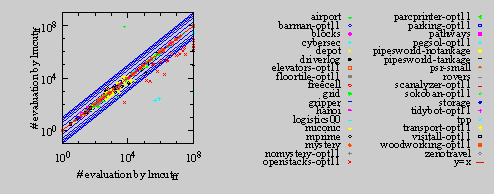
\includegraphics{tables/aaai16-30min/aaai16prelim3/evaluated-lmcut_ff-lmcut_lf.pdf}
 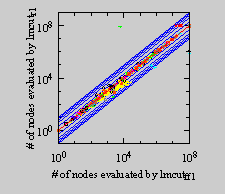
\includegraphics{tables/aaai16-30min/aaai16prelim3/evaluated-nokey-lmcut_ff-lmcut_r.pdf}
 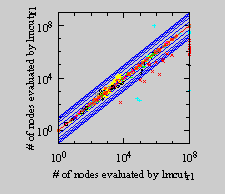
\includegraphics{tables/aaai16-30min/aaai16prelim3/evaluated-nokey-lmcut_r-lmcut_lf.pdf}
 \caption{Comparisons of \# of Evaluations between simple \lifo, \fifo,
 \ro second-level tiebreaking, with first-level $h$-tiebreaking. Each
 line shows $\times 2,4,6\ldots$ boundary.}  \label{f-h-eval}
\end{figure}

According to \reftbl{single-coverage} (left) with $h$-tiebreaking, \lifo
outperforms the other strategies, but Random Order outperforms the others in
Cybersec, and \fifo performed best in Airport, and
\refig{f-h-eval} shows that Random performs best in Miconic.
\refig{f-h-eval} also shows that the difference in number of nodes evaluated can sometimes be larger than a factor of 10,
especially in Openstacks and Cybersec.
Although \lifo second-level tie-breaking appears to perform best overall on these benchmarks, 
there are no dominance relationship between these three strategies, and the overall performance of each strategy will depend on the composition of problem instances in the benchmark set.
%These differences are purely due to the domain characteristics. 

\subsubsection{Is $h$-Based Tie-Breaking necessary?}

Next, we investigated whether $h$-based, first-level tie-breaking is necessary.
In \reftbl{single-coverage} (right), which shows the results when  first-level
tiebreaking based on $h$ is disabled, $[f, \lifo]$, which simply breaks ties among nodes with the same $f$-cost by expanding most recently generated nodes first (first suggested in \cite{korf1985depth}),
clearly dominates $[f, \fifo]$ and $[f, \ro]$.

Interestingly, the performance of the $[f, \lifo]$ strategy
is comparable to $[f,h,\lifo]$, $[f,h,\fifo]$ and $[f,h,\ro]$, the two-level strategies that first break ties according to $h$.
This is somewhat surprising, considering the ubiquity of $h$-based tie-breaking in the search and planning communities.
\todo{Explanation of why $[f,\lifo]$ performs so well. }
% 
This can be understood as \lifo greedily explores the plateau space
and quickly aggregates the $g$ value. Since $f$ is fixed within the
plateau, it also means $h$ decrease quickly, resulting in the similar behavior.

% We reemphasize that, although \lifo dominated the others, we consider
% this is just by a coincidence due to the selection of time limit, memory
% limit and problems in the current standard IPC competition
% settings. \emph{We are not trying to claim that any of \lifo or \fifo or
% Random order always dominates the others}.

% However, there are noticeable
% performance difference caused by these different tiebreaking strategies.

\subsubsection{Plateaus and Tie-Breaking}

In our comparison of the simple two-level tie-breaking strategies
above, we observed that large differences in performance between
two-level tie-breaking strategies tend to occur in problems where
there are many nodes that have the same $f$ and $h$ values, creating
large plateau regions where the heuristic does not provide
useful guidance -- in effect, these plateau regions in the last
frontier ($f=f^*$) by definition requires blind search, i.e., 
relying solely on the tie-breaking criterion, in order to
%% in the final plateau, there is no need to escape the
%% plateau. ``escape'' is a word for inadmissible search. A* is never
%% allowed to escape the plateau until all nodes are expanded.
% escape the plateau and
find a goal node.
%, i.e., the problems where the
%heuristic function is not informative and the planner relies heavily on
%the tiebreaking criteria.

\refig{plateau} plots the size of the final search plateau on 1104 IPC
benchmark instances \emph{with $h$-tiebreaking}.
The $y$-axis
represents the number of nodes with $[f,h]=[f^*,0]$, and the $x$-axis represents the total
number of nodes with $f\leq f^*$.
Clearly, in some domains such as Openstacks and Cybersec, the planner can spend most of the runtime
searching the final plateau.
It also
means that these domains have very large variance in the runtime caused
by the difference in second-level tiebreakings. 

%% Removed
% \refig{fig:plateau-noh} in the introduction is the same figure without $h$-tiebreaking.
% As expected, when the
% $h$-based tiebreaking is disabled in \refig{fig:plateau-noh}, much
% larger effort could be spent on the final plateau.

%  The size of the bucket does not change
% between $[f,h,\fifo]$, $[f,h,\lifo]$ and $[f,h,\ro]$.


\begin{figure}[tb]
 \centering \relsize{-3}
  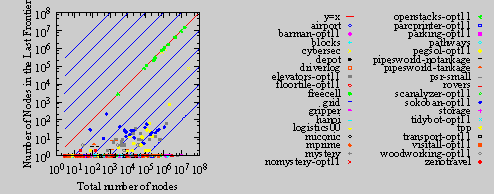
\includegraphics{tables/aaai16-frontier/aaai16prelim3/lmcut_frontier-front.pdf}
  \caption{Comparing the size of the $[f,h]$ search plateau to the total
  evaluation below $f\leq f^*$. Data were obtained by the result of
  \lmcut on the standard benchmark instances. Both axes are
  logarithmic. Dotted lines represent $\times 10^n$ boundaries.
  Openstacks clearly has the large plateaus.}  \label{plateau}
\end{figure}

\section{Domains with Zero-cost Actions}

Openstacks domain is a cost
minimization domain first introduced in IPC-2006, where the objective is to 
minimize the number of stacks used.
There are many zero-cost actions (i.e., actions that don't increase the number of stacks), and
these zero-cost actions prevent the commonly used heuristics from producing
informative guidance, confounding commonly used heuristics.
For example, \lmcut \cite{Helmert2009} fails to find a good cost
partitioning with non-zero values, 
% A detailed discussion of Openstacks domain and poor performance of landmarks is in \cite{richter10lama}, p.167-169.
and most edges in the abstraction
space of M\&S have zero costs \cite{helmert2007flexible}.

% XXX I'm commenting out the paragraphs below because:
% (1) A review of heuristic functions for domain-independent learning is not really
% necessary for this AAAI submission. 
% (2) It's better if this paper is not so strongly associated with the ICAPS community only -- this work applies in general to search with A*, and is not strongly tied to almost-perfect heuristics, lmcut, m&s, etc.

This kind of cost-minimization domains with many zero-cost actions are
not common in the current set of benchmark domains.
% 
Historically, the study of the shortest path finding algorithms has
started on the unit cost domains as the simplest case, where every
search edge has a cost 1,
% . Experimental study of \astar was somewhat biased to
% the unit-cost domains
such as 24-puzzle, Rubik's Cube etc.
There are also several problems with non-unit costs, sometimes
artificially but also sometimes naturally, such as in multiple
sequence alignment (MSA).
% 
In the plannning community, actions with non-unit costs were first introduced in 
IPC-2002. The actions in these domains tend to have the nonzero positive costs
because they mostly targets the runtime minimization.
% For example, Elevator and Miconic in the benchmark domains minimize the
% runtime of moving the passengers up and down.
% Actions in which the
% elevator travels the long distance take longer runtime.  
When concerned
only with the runtime, it is reasonable to assign nonzero positive cost to
every actions, since every actions are supposed to at least consume a
fraction of time.
However, such formulation is not suitable for the general minimization
problems.
For example, when you try to minimize the energy consumption
by the elevators in Elevators domain, many actions would have zero-cost
--- it does not consume electricity for either boarding or leaving the
passenger, or moving the elevator down.

As shown in the previous section, such domains pose a
difficulty to the current heuristic planners since they have large plateau.
Also, from the practical point of
view, cost minimization domains would have wider interest compared to
the simple runtime minimization.
% 
Therefore, in this paper, we modified various domains to have many
zero-cost actions.  For example, elevators-up is a variation of
Elevators domain which minimizes
the energy consumption caused by ``up'' action, which moves the elevator
up, and all other actions have zero-cost.  Modification was done in a
practically reasonable manner in a sense of cost minimization. Most
transportation-type domains are modified so that they use less
fuel (Logistics-fuel etc.). Assembly-type domains are modified so that it minimizes the
resource usage (floortile-ink minimizes ink usage, or Woodworking-cut
minimizes wood usage).
We call this set of domains as zerocost domains hereafter.

% \todo[We also modify a same domain
% in the different minimization criteria, in order to avoid the bias on a
% particular domain formulation.]{It's not tested yet}

% This lack of general support for cost-minimization problems
% in the current competition domains can be fixed by
% % The same thing applies to the transportation-type and assembly-type
% % domains like Logistics and Woodworking, respectively. They are runtime
% % minimization domains in which driving and manual labor, or cutting and
% % painting, are equally measured by the single runtime metric.
% modifying some actions to have zero-cost.
% For example, Logistics and Woodworking, in which driving and manual labor, or cutting and
% painting, are equally measured by the single runtime metric,
% can be converted into
% cost-minimization domains in which the target is the fuel consumption
% (Logistics) or wood usage (Woodworking). 


% Currently, most benchmark domains except Openstacks and Cybersec do not
% have the large plateau thanks to the powerful heuristic estimates (which
% is verified in the later section). However, limiting our effective
% experiments only to 2 domains would bias our observation. To avoid this
% issue, we created several domains where the \sota heuristic functions
% fail to provide a menaingful guidance.

% One important characteristics shared by Openstacks and Cybersec is that they both
% have large number of zero-cost actions.
 % In such situations, both LMcut
% and M\&S fail to find a meaningful heuristic estimate because LMcut fails to
% find a good cost partitioning with non-zero values, and most edges in the abstraction space of
% M\&S have zero costs.

% We therefore modified various domains to have many zero-cost actions.
% For example, miconic-up is a domain which minimizes the energy
% consumption caused by ``up'' action, which moves the elevator up, and
% all other actions have zero-cost. Another example is driverlog-fuel, where only
% the ``drive'' action has cost 1 and all other actions are zero-cost.
% This in fact reflects the practical application compared to the original
% unit-cost domains where driving and manual labor is equally accounted.
% Oddly, although some planners have options which treats actions as if
% they are unit-costs, and describe such options as ``inadmissible'',
% solving domains which are unit-cost by origin is not called
% ``inadmissible''. Above modification addresses this problem.

We plotted the size of plateau of the zerocost domains just like in
\refig{plateau}. The trend of large plateau becomes universal among
instances. In these cost-minimization problems, the search strategy within
plateau becomes much more important than in the
runtime-minimization problems.

\begin{figure}[tb]
 \centering \relsize{-3}
  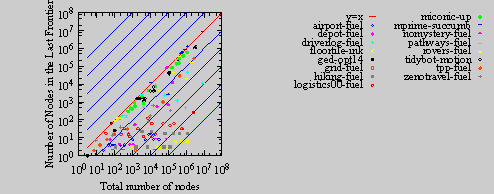
\includegraphics{tables/aaai16-frontier/zerocost/lmcut_frontier-front.pdf}
  \caption{Same plot as \refig{plateau}, but from the zerocost
  domains. Even with $h$-tiebreaking, zerocost domains force the planner
  to search much larger plateau.}
 \label{plateau-zerocost}
\end{figure}



\section{Depth-based Tiebreaking}

In order to solve problems with large final plateaus, the
planner needs to run an efficient knowledge-free search within the
plateau.  One useful notion which can be used to both understand and control the search in this
situation is the \emph{depth} of a node, which represents the number 
of steps from the entrance of the plateau.
If the $parent(n)$ is from the other plateau, i.e., $parent(n)$ has a
different $f$-value, or different $h$-value used for the first
tiebreaking, then $depth(n) = 0$. Nodes with $depth(n) = 0$ are called
the \emph{entrance} of the plateau.
If the $parent(n)$ is from the same plateau i.e.\ $parent(n)$ and $n$
shares the same $f$ and $h$,
$depth(n)$ is defined as $depth(parent(n)) + 1$.
Based on this simple notion of depth,
we propose  \emph{depth-based tie-breaking}, where all nodes are associated with its depth, 
and depth is used as a tie-breaking criterion.
FirstDepth(\fd), RandomDepth(\rd) and LastDepth(\ld) breaks ties by choosing a node from 
nodes with the smallest depth, a random depth, or the largest depth, respectively.

Since there can be multiple nodes with the same $f$, $h$ and depth,
a further tie-breaking criterion is necessary to select among nodes in the same depth bucket.
A natural 3rd-level tie-breaking policy is Random Order (\ro), which randomly selects an element from the depth bucket selected by the 2nd-level depth-based tie-breaking.
We consider the following 3 tie-breaking configurations, each using $h$
as the first-level tie-breaking criterion, one of \fd, \rd, \ld as the
depth-based 2nd-level tie-breaking criterion, and \ro as the 3rd-level
criterion:  $[f,h,\fd,\ro]$, $[f,h,\ld,\ro]$, $[f,h,\rd,\ro]$. 
In addition, we will also consider two additional configurations, $[f,h,\fd,\fifo]$, which is equivalent to $[f,h,\fifo]$, and $[f,h,\ld,\lifo]$, which is equivalent to $[f,h,\lifo]$.\footnote{
%Also note that, the node evaluation orders of $[f,h,\fd,\fifo]$ and $[f,h,\ld,\lifo]$ are
%exactly the same as $[f,h,\fifo]$ and $[f,h,\lifo]$, respectively,
%i.e., those without the depth-based tiebreaking.  
This is because, $[f,h,\lifo]$ expands the most recently evaluated/inserted
states, which always have the largest depth, and $[f,h,\fifo]$ expands the oldest
evaluated states, which always have the smallest depth.}
Thus, we consider five, 3-level configurations in all.


The effectiveness of each strategy depends on the structure of the problem instance.
In the knowledge-free search within the plateau, all nodes have the same
$f$ and $h$ values % yes, for simplicity, I'm assuming 3-level tiebreaks, ignoring no-h for the time being..
 and it is impossible to guess whether the goal is near, far
away or in a particular distance from the entrance.
In the first case,
the search should be focused around the entrance favoring the smaller
depths (FirstDepth), and the behavior should be much like breadth-first. In the second case, the planner should
greedily explore the various area of the plateau by preferring larger
depth (LastDepth), much like in depth-first. In the
final case where the goal node is in a particular depth, choosing the
random depth seems the safest practice. This corresponds to the case
where RandomDepth would perform better.

% This ``greediness'' is different from the normal
% sense of ``greedy search'' --- since this greediness only holds within
% the plateau, admissibility is still maintained.
 


\subsection{Evaluating Depth-based Tiebreaking}

We evaluated the five, 3-level tie-breaking strategies described above.
%REDUNDANT? , i.e., $[f,h,depthStrategy,LFR]$, where the first-level tie-breaking is according to $h$ (break ties in favor of small $h$), the second-level strategy is based on depth and $depthStrategy \in \{\fd, \ld, \rd\}$, and the third level tie-breaking strategy $LFR \in \{\lifo, \fifo, \ro\}$.
% 
In addition to the 28 standard IPC benchmark domains used in the previous set of experiments, we also added 16 \emph{zerocost} domains with 640 problems. 

The node evaluation order of $[\cdot,\fd,\fifo]$ and $[\cdot,\ld,\lifo]$
are exactly the same as those without the second-level
depth-based tiebreaking, i.e.\ $[\cdot,\fifo]$ and $[\cdot,\lifo]$.
Yet these results are useful in assessing the extra cost of managing the
depth-based buckets.

\refig{depth} shows various experiments on benchmark domains and
zerocost domains. Regardless of the third-level tiebreaking, LastDepth
strategy tends to be dominant in most domains. However, RandomDepth and
FirstDepth still exhibits a significantly better performance in Cybersec
and Mistery-Feast, respectively, indicating there is no true dominance relationship.

This result explains why the simple $[f,h,\lifo]$ strategy has become
successful. $[f,h,\lifo]$ is same as $[f,h,\ld,\lifo]$, and the fact
that the performance of $[f,h,\ld,\cdot]$ was consistently good
regardless of the third-level tiebreaking means that the performance of
$[f,h,\ld,\lifo]$ was caused by LastDepth and not by third-level \lifo tiebreaking.

Supporting the above claim, the overall dominant third-level tiebreaking
in these experiments is \fifo.  For example, when we fix the second-level
tiebreaking, the coverages are $[f,h,X,\fifo]>[f,h,X,\ro]>[f,h,X,\lifo]$
when $X=\ld,\rd$.  Note that \fifo is bad in terms of low-level memory
access pattern since the insertion and deletion happens in the opposite
side of the bucket. 

Note that we do not claim the performance of \fifo in third-level
tiebreaking is universal.  Rather, it is more likely due to the specific
action ordering in the domain definition. \todo[First]{thise text should
be adjusted after 30min results}, in Pipesworld-Pushend,
for example, the dominant third-level strategy is RandomOrder,
regardless of the second-level depth tiebreaking.  (\fifo,\ro,\lifo is
3,3,3 in FirstDepth, 3,4,3 in RandomDepth, and 5,6,4 in LastDepth.)
Also, in Airport-Fuel and Mprime-Succumb with RandomDepth ($[f,h,\rd,\cdot]$), 
the RandomOrder third-level tiebreaking is better than \lifo or \fifo.
Furthermore, we also tested the same domains with a reversed
action ordering. The results (in supplimental
material) show that the action ordering affects the performance of
third-level tiebreaking, but it did not changed the trends in the
second-level tiebreaking.

This third-level tiebreaking behavior is related to recent work
\cite{vallati2015effective} done by changing the action and variable
ordering with SMAC parameter tuning framework. However, finding the best
third-level tiebreaking is not the scope of this paper.

%% following discource may not be a good way to defend our paper.
% Keen readers might be concerned with the effect of action ordering in
% the domain definition. Although we showed that tie-breaking makes a
% difference, all the minor differences could be accidental and due to the
% input ordering, i.e., tiebreaking could change their behavior in some
% cases by changing the sort order of the actions.
% 
% This consideration does not diminish our depth-based second tiebreaking.
% First, the only part affected by the action ordering is the
% third tiebreaking, for which we tested \lifo, \fifo and \ro.
% We are not trying to claim some dominance relationships within these
% third tiebreakings. The purpose of the comparison 

% also, even with 2-level tiebreaking,  2nd level random tiebreaking, lmcut(f,r), did not perform that well, so that supports the claim that re-ordering alone cannot explain all the results, and lmcut(f,h,r) is significantly worse than lmcut(f,h,lifo).

% Another issue in this result is the lack of analysis on
% abstraction-based heuristics. We also added the results in the figures
% in the supplemental materials. Above trends are mostly consistent when
% M\&S and blind heuristics are used, regardless of first-level
% tiebreaking by $h$-value. However, we note that many instances quickly
% exhausted the 2GB memory limit with those heuristics, and is less
% informative compared to the result by LMcut.

\begin{figure}[htb]
 \centering
 \relsize{-3}
 \begin{tabular}{|c|c|c|c|c|c|c|c|c|c|}
\hline                           
 Domain & \rotatebox[origin=l]{90}{${\mbox{lmcut}}_{\mbox{${\mbox{fd}}_{\mbox{fifo}}$}}$}   & \rotatebox[origin=l]{90}{${\mbox{lmcut}}_{\mbox{${\mbox{rd}}_{\mbox{fifo}}$}}$}   & \rotatebox[origin=l]{90}{${\mbox{lmcut}}_{\mbox{${\mbox{ld}}_{\mbox{fifo}}$}}$}   & \rotatebox[origin=l]{90}{${\mbox{lmcut}}_{\mbox{${\mbox{fd}}_{\mbox{random}}$}}$}   & \rotatebox[origin=l]{90}{${\mbox{lmcut}}_{\mbox{${\mbox{rd}}_{\mbox{random}}$}}$}   & \rotatebox[origin=l]{90}{${\mbox{lmcut}}_{\mbox{${\mbox{ld}}_{\mbox{random}}$}}$}   & \rotatebox[origin=l]{90}{${\mbox{lmcut}}_{\mbox{${\mbox{fd}}_{\mbox{lifo}}$}}$}   & \rotatebox[origin=l]{90}{${\mbox{lmcut}}_{\mbox{${\mbox{rd}}_{\mbox{lifo}}$}}$}   & \rotatebox[origin=l]{90}{${\mbox{lmcut}}_{\mbox{${\mbox{ld}}_{\mbox{lifo}}$}}$}    \\
\hline                           
 sum(1104) &  600 &  612 &  612 &  598 &  613 &  610 &  602 &  \textbf{615} &  606  \\
\hline                           
 {\relsize{-1}airport(50)} &  \textbf{28} &  \textbf{28} &  \textbf{28} &  27 &  27 &  27 &  27 &  27 &  27  \\
 {\relsize{-1}cybersec(19)} &  2 &  8 &  9 &  2 &  10 &  7 &  4 &  \textbf{12} &  3  \\
 {\relsize{-1}mprime(35)} &  22 &  22 &  22 &  22 &  22 &  22 &  \textbf{23} &  \textbf{23} &  \textbf{23}  \\
 {\relsize{-1}openstacks-opt11(20)} &  13 &  \textbf{19} &  \textbf{19} &  12 &  \textbf{19} &  \textbf{19} &  13 &  \textbf{19} &  \textbf{19}  \\
 {\relsize{-1}pipesworld-tankage(50)} &  \textbf{12} &  \textbf{12} &  11 &  \textbf{12} &  \textbf{12} &  \textbf{12} &  \textbf{12} &  11 &  11 \\
\hline
 sum(380) &  174 &  186 &  \textbf{189} &  170 &  184 &  \textbf{189} &  173 &  179 &  179  \\
\hline                           
 {\relsize{-1}airport-fuel(20)} &  \textbf{17} &  16 &  \textbf{17} &  15 &  15 &  16 &  16 &  \textbf{17} &  15  \\
 {\relsize{-1}driverlog-fuel(20)} &  \textbf{9} &  8 &  8 &  8 &  \textbf{9} &  8 &  \textbf{9} &  8 &  8  \\
 {\relsize{-1}floortile-ink(20)} &  9 &  9 &  9 &  9 &  9 &  9 &  9 &  \textbf{10} &  9  \\
 {\relsize{-1}miconic-up(30)} &  17 &  22 &  22 &  17 &  \textbf{23} &  \textbf{23} &  17 &  21 &  22  \\
 {\relsize{-1}mprime-succumb(35)} &  18 &  24 &  \textbf{27} &  18 &  22 &  26 &  18 &  15 &  17  \\
 {\relsize{-1}pathways-fuel(30)} &  \textbf{5} &  \textbf{5} &  4 &  4 &  4 &  4 &  \textbf{5} &  \textbf{5} &  \textbf{5}  \\
 {\relsize{-1}tpp-fuel(30)} &  8 &  11 &  11 &  8 &  11 &  \textbf{12} &  8 &  \textbf{12} &  \textbf{12} \\
\hline
 sum(260) &  124 &  140 &  147 &  122 &  149 &  \textbf{150} &  124 &  149 &  144  \\
\hline                           
 {\relsize{-1}elevators-up(20)} &  7 &  10 &  12 &  7 &  11 &  11 &  7 &  \textbf{13} &  \textbf{13}  \\
 {\relsize{-1}freecell-move(20)} &  5 &  17 &  \textbf{20} &  5 &  19 &  \textbf{20} &  5 &  18 &  19  \\
 {\relsize{-1}gripper-move(20)} &  \textbf{7} &  \textbf{7} &  \textbf{7} &  6 &  6 &  6 &  \textbf{7} &  \textbf{7} &  \textbf{7}  \\
 {\relsize{-1}mystery-feast(20)} &  \textbf{9} &  8 &  8 &  \textbf{9} &  \textbf{9} &  \textbf{9} &  \textbf{9} &  \textbf{9} &  \textbf{9}  \\
 {\relsize{-1}pipesnt-pushstart(20)} &  10 &  \textbf{11} &  \textbf{11} &  10 &  \textbf{11} &  \textbf{11} &  \textbf{11} &  10 &  10  \\
 {\relsize{-1}pipesworld-pushend(20)} &  4 &  4 &  8 &  5 &  \textbf{10} &  \textbf{10} &  5 &  9 &  7  \\
 {\relsize{-1}psr-small-open(20)} &  19 &  19 &  \textbf{20} &  19 &  19 &  19 &  19 &  \textbf{20} &  19  \\
 {\relsize{-1}scanalyzer-analyze(20)} &  \textbf{11} &  \textbf{11} &  9 &  \textbf{11} &  \textbf{11} &  9 &  \textbf{11} &  \textbf{11} &  9  \\
 {\relsize{-1}sokoban-pushgoal(20)} &  \textbf{20} &  \textbf{20} &  19 &  \textbf{20} &  \textbf{20} &  19 &  \textbf{20} &  \textbf{20} &  19  \\
 {\relsize{-1}storage-lift(20)} &  5 &  5 &  \textbf{6} &  5 &  5 &  \textbf{6} &  5 &  5 &  5  \\
 {\relsize{-1}woodworking-cut(20)} &  7 &  8 &  7 &  5 &  8 &  \textbf{10} &  5 &  7 &  7 \\
\hline
 total(1744) &  898 &  938 &  948 &  890 &  946 &  \textbf{949} &  899 &  943 &  929 \\
\hline
\end{tabular}

 \caption{Experiments
 comparing the coverages of 9 configurations (3 depth-based strategy
 $\times$ 3 queue implementions). For the space reason, we omitted those
 domains whose results are the same. (Full results are available in the
 supplemental material.) Each cell denotes the problem solved with 30
 min, 2GB setting. \textbf{Boldface} denotes the case where it achieved
 the best result among configurations. Zerocost domains are named
 according to [original]-[name of nonzero action].}
 \label{depth}
\end{figure}

%% obviously does not fit in the paper
% \begin{figure}[htb]
%  \centering
%  \relsize{-3}
%  \begin{tabular}{|c|c|c|c|c|c|c|c|c|c|}
\hline                           
 Domain & \rotatebox[origin=l]{90}{${\mbox{lmcut}}_{\mbox{${\mbox{fd}}_{\mbox{${\mbox{fifo}}_{\mbox{noh}}$}}$}}$}   & \rotatebox[origin=l]{90}{${\mbox{lmcut}}_{\mbox{${\mbox{rd}}_{\mbox{${\mbox{fifo}}_{\mbox{noh}}$}}$}}$}   & \rotatebox[origin=l]{90}{${\mbox{lmcut}}_{\mbox{${\mbox{ld}}_{\mbox{${\mbox{fifo}}_{\mbox{noh}}$}}$}}$}   & \rotatebox[origin=l]{90}{${\mbox{lmcut}}_{\mbox{${\mbox{fd}}_{\mbox{${\mbox{random}}_{\mbox{noh}}$}}$}}$}   & \rotatebox[origin=l]{90}{${\mbox{lmcut}}_{\mbox{${\mbox{rd}}_{\mbox{${\mbox{random}}_{\mbox{noh}}$}}$}}$}   & \rotatebox[origin=l]{90}{${\mbox{lmcut}}_{\mbox{${\mbox{ld}}_{\mbox{${\mbox{random}}_{\mbox{noh}}$}}$}}$}   & \rotatebox[origin=l]{90}{${\mbox{lmcut}}_{\mbox{${\mbox{fd}}_{\mbox{${\mbox{lifo}}_{\mbox{noh}}$}}$}}$}   & \rotatebox[origin=l]{90}{${\mbox{lmcut}}_{\mbox{${\mbox{rd}}_{\mbox{${\mbox{lifo}}_{\mbox{noh}}$}}$}}$}   & \rotatebox[origin=l]{90}{${\mbox{lmcut}}_{\mbox{${\mbox{ld}}_{\mbox{${\mbox{lifo}}_{\mbox{noh}}$}}$}}$}    \\
\hline                           
 sum(1104) &  0 &  0 &  0 &  0 &  0 &  0 &  0 &  0 &  0  \\
\hline                           \\
\hline
 sum(380) &  0 &  0 &  0 &  0 &  0 &  0 &  0 &  0 &  0  \\
\hline                           \\
\hline
 sum(260) &  0 &  0 &  0 &  0 &  0 &  0 &  0 &  0 &  0  \\
\hline                           \\
\hline
 total(1744) &  0 &  0 &  0 &  0 &  0 &  0 &  0 &  0 &  0 \\
\hline
\end{tabular}

%  \caption{Same experiments without first-level tiebreaking by $h$-value.}
%  \label{depth-noh}
% \end{figure}

\section{Low-Overhead Portfolios for Combining Tie-Breaking Strategies}

As noted above, it is unknown prior to the search where the goal node
exists in a plateau.
However, the best tiebreaking strategy seems to be affected by the domain
characteristics, as we show in the evaluation section.

Since the performance of a tiebreakig strategy depends on the domain, and there is no clear dominance relationship among the tiebreaking strategies, one natural 
idea is to use a portfolio approach which combine several tiebreaking strategies.

The simplest possible portfolio approach would be a standard algorithm portfolio
which executes two completely independent \astar processes $A_1$ and $A_2$ in parallel, where $A_1$ uses tiebreaking strategey $S_1$ and $A_2$ uses tiebreaking strategy $S_2$, and CPU resources are allocated equally to $A_1$ and $A_2$.
The portolio would terminate when either $A_1$ or $A_2$ finds a goal state.
Let $T_1$ be the time that $A_1$ requires to solve instance $I$, and $T_2$ be the
time $A_2$ requires to solve instance $I$. Then, the total CPU time
required by the portfolio to solve instance $I$ is $2\times\min(A_1,A_2)$. This approach to combining multiple strategies is the standard algorithm portfolio proposed and analyzed in \cite{HubermanLH97,GomesS01}, and has also recently been called ``dovetailing'' and applied to combine multiple IDA* and \astar  \cite{ValenzanoSSBK10}. %TODO: remove the dovetailing reference after the paper is accepted -- the dovetailing authors were unaware of the HubermanLH97 paper...

On one hand, this simple portfoio approach has the advantage of mitigating worst-case risk -- as shown in \refig{plateau}, sometimes, the ratio between $T_1$ and $T_2$ is very large (e.g., $T_2 > 10\times T_1$) and choosing the wrong strategy has a very high penalty, so this portfolio strategy guarantees that the CPU usage is never more than twice that of using the faster strategy.
On the other hand, this simple portfolio will always require twice the CPU time of the faster strategy. Furthermore, the portfolio requires twice the RAM resources, which is a major disadvantage in memory-bound algorithms such as \astar.

We propose a new, \emph{Low-Overhead Portfolio} (LOP) implementation which can be used to implement a portfolio of tie-breaking strategies with significantly less overhead.
% 
Conceptually, a LOP for \astar is a portfolio composed of multiple
independently executing \astar where each \astar has completely separate
open/closed list, using a different tiebreaking strategy but sharing a
global cache for heuristic function values. Whenever a search engine
evaluates a state, it first checks the cache and reuses the result if
possible.  The current implementation is sequential -- each search
engine takes turns evaluating states. The algorithm finishes when some
engine finds the solution. Note that it does not \emph{expand} states in
turns --- in that case, the number of evaluation would be affected by
the difference in the number of successor states of each node and the
evaluation effort would not be evenly distributed. There is a small pool
storing the nodes which are expanded but not yet evaluated. Evaluation
happens in turns, and if the pool is exhausted, the expansion occurs as
necessary in order to evaluate more nodes.

Low-Overhead Portfolios offer some attractive tradeoffs,
particularly when runtimes are dominated by state evaluation, as is the case when searching with 
expensive heuristics such as LM-cut or recently proposed LP-based heuristics \cite{PommereningRHB14,ImaiF14}.

First, although the effort to insert/extract nodes from multiple open/closed lists is also doubled, these overheads
are neglibigle when the heuristic is expensive (see \refig{ffff},left).

Second, although maintaining multiple open/closed lists requires additional memory,
when the heuristic is expensive enough, runtime becomes a bigger issue
than memory exhaustion  -- we show that with a 30 minute time limit, LOP
configurations do not exhaust memory more often than the other
configurations does \refig{ffff}(right).

Third, node evaluation overheads for $f < f^*$ are eliminated due to the $h$-cache.
Recall that \astar always evaluates all states whose $f$ costs 
below $f^*$. Since the heuristic function $h$, and in turn $f=g+h$, is
the same among the tiebreaking strategies, they evaluate the same set of
nodes with $f<f^*$, so unlike a standard portfolio implementation where 
nodes with $f<f^*$ would be evaluated multiple times, there is no evaluation overhead in a LOP
for nodes with $f<f^*$.
Note that this is not
affected by the reopening of the node caused by inconsitent heuristics
since the $h$-value is cached.

%% Third, since the search terminates when \emph{some} engine finds a
%% solution, and since the evaluation happens in turns, the search effort
%% within the final plateau is upper bounded by \emph{twice} the
%% \emph{minimum} of the search efforts required by each of \ld-\lifo or
%% \ld-\fifo engine alone.  Evaluating the same nodes in different engines
%% also reduces the effort to less than twice due to caching.  This is
%% desirable because, as we saw in the Results section, in some domains the
%% gap between the best and worst tiebreaking strategy can be more than 10
%% times (Openstacks, for example).  When there are $n$ engines, then this
%% increases to $n\times$ minimum amount of effort which would be spent by
%% each single engine alone.

Finally, in the worst case, the total number of nodes evaluated by a LOP is bounded by the number of nodes with $f \leq f^*$, which is the same as the worst-case behavior of \astar using the worst possible tie-breaking strategy.
This can occur  when all tiebreaking
strategies perform poorly  and they all evaluates the goal node in the
final iteration.

\subsection{Evaluating LOPs}

As we see in the previous section, the planner performance is greatly
affected by the tiebreaking criteria, especially when the search plateau
is huge, which is more often the case with the more practical,
cost-minimization domains.
% 
Also, the different depth-based tiebreakings are not dominating
each other and is unpredictably affected by the domain characteristics.
% 
Therefore, the LOP strategy should avoid the
worst-case scenario caused by bad tiebreaking, and quickly find the solution.

First, we show that the doubled cost of insertion and deletion by LOP is
negligeble.  We verified this by comparing the runtime of single \astar
with a LOP consisting of two same \astar, where all three \astar{}s
using the idential configuration ($[f,h,\fifo]$ with $h=$\lmcut). The
result in \refig{ffff} shows that the extra cost of duplicated effort
is negligeble.

\begin{figure}[htb]
 \centering \relsize{-2}
 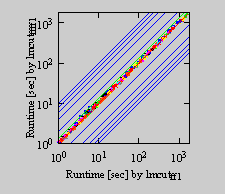
\includegraphics{tables/aaai16-30min/aaai16prelim3/time-nokey-lmcut_ff-lmcut_ffff.pdf}
 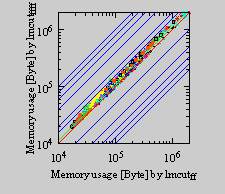
\includegraphics{tables/aaai16-30min/aaai16prelim3/mem-nokey-lmcut_ff-lmcut_ffff.pdf}
 \caption{Comparison of the runtimes (left) and memory usage (right) by
 single $[f,h,\fifo]$ and a LOP engine with 2 different instances of
 $[f,h,\fifo]$. Each line shows $\times 2,4,6\ldots$ boundary.
 The runtime and memory usage difference were at most a factor of x1.3
 and x1.6 (shown in green line) and in most cases lower than that. We
 ignore the subsecond differences.}  \label{ffff}
\end{figure}

Next, we evaluated our LOP
strategy with selective combinations of two or three tiebreakings.
The configuration shown as ``lmcut m2'', ``lmcut m3'', ``mands m2'',
``lmcut m3'' are respectively the portfolio of
$[\ld,\fifo]$ + $[\rd,\lifo]$, $[\ld,\fifo]$ + $[\ld,\ro]$ + $[\rd,\lifo]$,
$[\ld,\fifo]$ + $[\rd,\ro]$, $[\ld,\fifo]$ + $[\rd,\ro]$ + $[\ld,\lifo]$. These
portfolios are selected by hand based on the previous results.
% LOP is able to avoid the accidental bias
Results in \reftbl{portfolio-coverage}
shows a significant improvements compared to the results by each search
engine alone.
% 
Also, \refig{portfolio-runtime} shows the number of evaluations of these
tiebreakings compared to each search engine alone.  It shows that
LOP acutally follows the expected behavior and the theoretical
bounds: the evaluation never exceeds twice/thirds of the single
search engine.

\begin{table}[htb]
 \centering \relsize{-2}
 \begin{tabular}{|c|c|c|c|}
\hline         
 Domain & \rotatebox[origin=l]{90}{${\mbox{lmcut}}_{\mbox{${\mbox{rd}}_{\mbox{random}}$}}$}   & \rotatebox[origin=l]{90}{${\mbox{lmcut}}_{\mbox{${\mbox{ld}}_{\mbox{random}}$}}$}   & \rotatebox[origin=l]{90}{${\mbox{lmcut}}_{\mbox{${\mbox{ldrd}}_{\mbox{random}}$}}$}    \\
\hline         
 sum(1104) &  \textbf{613} &  610 &  \textbf{613}  \\
\hline         
 {\relsize{-1}cybersec(19)} &  10 &  7 &  \textbf{11}  \\
 {\relsize{-1}gripper(20)} &  \textbf{7} &  \textbf{7} &  6 \\
\hline
 sum(380) &  184 &  \textbf{189} &  184  \\
\hline         
 {\relsize{-1}airport-fuel(20)} &  15 &  \textbf{16} &  \textbf{16}  \\
 {\relsize{-1}driverlog-fuel(20)} &  \textbf{9} &  8 &  8  \\
 {\relsize{-1}hiking-fuel(20)} &  \textbf{11} &  \textbf{11} &  10  \\
 {\relsize{-1}miconic-up(30)} &  \textbf{23} &  \textbf{23} &  22  \\
 {\relsize{-1}mprime-succumb(35)} &  22 &  \textbf{26} &  24  \\
 {\relsize{-1}tpp-fuel(30)} &  11 &  \textbf{12} &  11 \\
\hline
 sum(260) &  149 &  \textbf{150} &  147  \\
\hline         
 {\relsize{-1}elevators-up(20)} &  \textbf{11} &  \textbf{11} &  10  \\
 {\relsize{-1}freecell-move(20)} &  19 &  \textbf{20} &  \textbf{20}  \\
 {\relsize{-1}mystery-feast(20)} &  \textbf{9} &  \textbf{9} &  8  \\
 {\relsize{-1}pipesnt-pushstart(20)} &  11 &  11 &  \textbf{12}  \\
 {\relsize{-1}pipesworld-pushend(20)} &  \textbf{10} &  \textbf{10} &  9  \\
 {\relsize{-1}scanalyzer-analyze(20)} &  \textbf{11} &  9 &  10  \\
 {\relsize{-1}sokoban-pushgoal(20)} &  \textbf{20} &  19 &  19  \\
 {\relsize{-1}storage-lift(20)} &  5 &  \textbf{6} &  \textbf{6}  \\
 {\relsize{-1}woodworking-cut(20)} &  8 &  \textbf{10} &  8 \\
\hline
 total(1744) &  946 &  \textbf{949} &  944 \\
\hline
\end{tabular}

 \caption{Coverage results comparing some LOP combinations and the
 single strategies under the portfolio. }
 \label{portfolio-coverage}
\end{table}

\todo{the evaluations are double-counted for LOP}

\begin{figure}[htb]
 \centering
 \relsize{-2}
 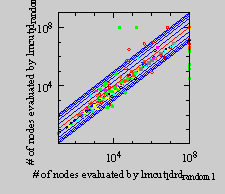
\includegraphics{tables/aaai16-30min/zerocost/evaluated-nokey-lmcut_ldrd_random-lmcut_ld_random.pdf}
 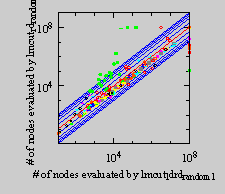
\includegraphics{tables/aaai16-30min/zerocost/evaluated-nokey-lmcut_ldrd_random-lmcut_rd_random.pdf}
 \caption{Comparson of runtimes between LOP $[\ld,\ro]$ +
 $[\rd,\ro]$ and the single strategy $[\ld,\ro]$ and $[\rd,\ro]$, on
 zerocost instances.}  \label{portfolio-runtime}
\end{figure}


\section{Related Work}
\label{sec-4}

Previous work on escaping search space plateaus has focused on
non-admissible search.  DBFS \cite{imai2011novel} is a technique which
adds stochastic backtracking to Greedy Best First Search to avoid
being misdirected by the heuristic function. Type based bucket
\cite{xie14type} classifies the plateau of GBFS according to the
$[g,h]$ pair.  Marvin \cite{Coles07} learns plateau-escaping macros
from the Enhanced Hill Climbing phase of the FF planner
\cite{Hoffmann01} and later uses these macros to escape the plateau.
However, to our knowledge, searching in plateaus has not been
previously investigated for cost-optimal planning with admissible
search.

In their work on combining multiple heuristics in a planner, R\"{o}ger
and Helmert considered a tie-breaking approach which works as follows:
\shortcite{RogerH10}. When combining two heuristics, one of the
heuristics is used as the primary criterion for guiding the search,
and the second heuristic is used to break ties when the primary
heuristic values are the same for two states.
While this did not perform well in their work on satisficing planning, 
using a secondary heuristic as a tie-breaking criterion in our multi-level tie-breaking framework 
for cost-optimal search is an interesting direction for future work.

The PLUSONE cost-type is  non-admissible search technique in the LAMA planner \cite{richter2010lama}
which increases every action costs by 1.\todo{Is PLUSONE mentioned in any paper??}
By eliminating zero-cost actions, this has the effect of filling plateaus
%Using PLUSONE, three successive
%applications of zero-cost operators have cost 3, and two
%applications have cost 2, and smaller cost is preferred, just as
%\astar always expands the node with smaller $f$-value.
This explicitly targeted zero-cost actions observed in Openstacks,
and resulted in a significantly better performance in IPC-6.\todo{citation? -- add specific page+quotation in comment}
% There's a long discussion of Openstacks in \cite{richter2010lama}, p.167-169, but I can't find PLUSONE anywhere. Maybe it's called something else in the paper?  Maybe \richter2010lama is the wrong citation??


The major difference of our depth-based tiebreaking from PLUSONE
strategy is twofold.  First, depth-based tiebreaking is admissible, because 
unlike PLUSONE, action costs are not modified.
Also, \emph{we do not always favor smaller depth over
larger depth}. LAMA treats the increased cost as the part of
sorting criteria. In contrast, it happens only in FirstDepth configuration in our case.

%% this will invoke a request from the reviewers to compare ours against it
%% * True, but people who know LAMA/FD are likely to demand some kind of comparison with alternating queues and preferred queues whether we mention  it or not.
%% Probably better to preemptively settle these questions rather than risking difficult questions during rebuttal.

Fast Downward and Lama implement an (OPEN) queue \emph{alternation}
method \cite{Helmert2006}.  It was originally used as a method for using
multiple heuristics in a planner.  There are multiple open lists
(queues), where there is a queue for each heuristic, and states are
inserted into all queues according to the heuristic value for each
heuristic.  The major difference of alternation queue to LOP is twofold:
First, LOP uses a single, expensive heuristic as the primary sorting
criteria ($f$-value), and it does not alternates between multiple
heuristics. Second, unlike alternation queue alternates the
\emph{expansion}, LOP alternates the \emph{evaluation}.

Preferred operator queues are an extension of queue alternation, where in addition to the basic queue for each heuristic, there is a queue for states that are \emph{preferred} according to each heuristic \cite{richter2010lama}.
Although this was designed for non-admissible search in LAMA, preferred operators could, in principle, be applied to admissible search. 
Preferred operators are implemented by adding operator (state) preference computation to heuristic evaluator, and are therefore dependent on the heuristic function.
% Evidence: \cite{richter2010lama}, p.132 ``Operators that are deemed particularly useful in a given state are marked as preferred.   They are computed by the heuristic estimators along with the heuristic value of a state (see Sections 6 and 5).  
% More Evidence: \cite{richter2010lama}, p.150, last paragraph: ``We also generate preferred operators along with the landmark heuristic. An operator is preferred in a state if applying it achieves an acceptable landmark in the next step, i. e., a landmark whose pre-decessors have already been accepted.  If no acceptable landmark can be achieved within one step, the preferred operators are those which occur in a relaxed plan to a nearest acceptable landmark. A nearest landmark in the cost-unaware setting is one that is relaxed reachable with a
In contrast, the tie-breaking strategies investigated in this paper are implemented completely independently of the heuristic -- all of the tie-breaking stratgies in this paper can be applied to search using a blind heuristic.

%Lazy A* \cite{TolpinBSFK13} 
%TODO:  lazy A* vs LOP -- LazyA* combines multiple heuristics h1,h2 with low-overhead. However, if there is no dominance between h1,h2, behavior is different than h2; in contrast, LOP guarantees conservative behavior. % no, never mind, too different..

% It's not clear what these techniques have in common, except that they are all orthogonal to heuristics,
% If that's the case, then there's no need to cite them in this paper -- there's no reason why these particular techniques
% are more relevant to this paper than hundreds of other techniques that are orthogonal to heuristics.
%% In admissible planning,
%% \emph{Symmetry Breaking}
%% \cite{Fox1998,pochter2011exploiting,domshlak2013symmetry} is the search
%% technique that tries to prune the states with symmetric
%% paths. \emph{Partial Order Reduction}
%% % , \emph{Strong Stubbern Sets} and \emph{Expansion Core} are
%% is also a technique which prunes the
%% intermediate states that reach to the same goal using the different
%% orders of same actions. \emph{Dominance Pruning} \cite{hall2013faster} is a
%% technique which prunes a state if it can be proven to be worse than the other nodes.
%% % 
%% These are usually not considered an attempt to improve the heuristic
%% estimates, however, in terms of \emph{Path-dependent globally admissible
%% heurisitics} \cite{karpas2012optimal}, a class of heuristics which is
%% admissible only on a particular optimal path, generalizes the above
%% techniques as assigining an infinite cost to some nodes on the other optimal paths.
%% % 
%% % From a slightly different category, Pathmax \cite{mero1984heuristic} and
%% % Bidirectional Pathmax \cite{felner2011inconsistent} are the techniques
%% % which converts an inconsistent heuristics into non-decreasing,
%% % consistent heuristics.
%% Thus, in a broad term, all of these methods are the
%% attempts to improve the heuristic estimates.
%% % Although in some particular
%% % case they may be able to return a perfect heuristics, they are still not
%% % always a perfect heuristics, implying that the plateau is unavoidable.
%% In contrast, our tiebreaking techniques aims specifically at the case
%% where the plateau is encountered and the planners are forced to run a
%% knowledge-free search.

$LA^*$ \cite{stern2010look} extends \astar by performing a
cost-bounded depth-first \emph{lookahead} from each node as it is generated.
Although this work was not done in the context of tie-breaking strategies, it is interesting to note that 
when the lookahead cost bound $k=0$ ($LA^*_0$ in their notation), only nodes with the same $f$-value as the current \astar frontier are expanded, which corresponds to a LastDepth strategy.


\citeauthor{Hoffmann05} gives a detailed analysis of the
structure of the search space in the benchmark domains which were
available in time of \citeyear{Hoffmann05}
\cite{Hoffmann05,Hoffmann14}. 
The analysis was focused on the plateaus and dead ends which occur duing the inadmissible search,
and also 


Vallati et al \shortcite{vallati2015effective} investigated the effect of the ordering of objects (including operators, predicates, etc. ) in PDDL domain models, and showed that orderings can have a significant impact on planner performance.
They conjectured that the reason for for the performance variations caused by object reordering is due to the impact reordering has on tie-breaking among nodes with the same best $f$-value.
% in \cite{vallati2015effective} p.7, col2, par#1
XXXTODOXXX:very important comparison...



\section{Conclusion}

In this paper, we proposed two novel tie-braking methods for the admissible search using \astar. We empirically showed that they improve the performance on various domains, and they are heuristic-agnostic improvements. We showed that they have a significant impact on the final step of the search in large plateau.
 % when the distribution of optimal solutions is not uniform within the open list.
% We also showed that this nonuniform distribution still appears when we have almost-perfect % heuristics.

Our method differs from the pruning techniques because we actually
do not prune any states, nor from the other general improvements to the
heuristic accuracy because we just change the evaluation order within the
same $f$, yet it address the fundamental problems in the limitation of
heuristic forward search.  Future work includes a development of learning
technique for adaptively altering the search behavior in the plateau.



